\documentclass[ucs]{beamer}
\usepackage{etex}

%\usepackage[ngerman]{babel}
%\usepackage[latin1]{inputenc}

\usepackage[utf8x]{inputenc}
\usepackage[all]{xy}
\usepackage{hyperref}
\usepackage{algorithm2e}
\usepackage{tikz}
\usepackage{listings}
\usepackage{xcolor}
\usepackage[absolute,overlay]{textpos}
\usepackage{graphicx} % Required for the inclusion of images
\usepackage{amsmath} % Required for some math elements 
\usepackage{ae} % Uml. im PDF-Verzeichnis
%\makeatletter

% to change colors
\newcommand{\fillcol}{green!20}
\newcommand{\bordercol}{black}

\setbeamercovered{transparent} 
\mode<presentation>{
	  \useoutertheme[subsection=false]{miniframes}
	    \useinnertheme{rectangles}
		   \usecolortheme{crane}
}


\title{A Lattice Boltzmann Method for immiscible multiphase flow simulations using the Level Set Method} % Title

\author{Lorenz Hufnagel, Daniel Zint} % Author name
\institute{BGCE Student Project}

\date{August 20th, 2015} % Date for the report

\begin{document}

\maketitle % Insert the title, author and date

\section{Motivation \& Introduction}

\begin{frame}
\frametitle{Multiphase flow}
Examples
\begin{itemize}
\item<1-> Liquid-liquid mixtures (e.g. oil in water) 
\item<2-> Gas-liquid mixtures (e.g. bubble dynamics)
\end{itemize}

\begin{tabular}{l l}
\begin{minipage}{0.4\textwidth}

\visible<1->{
\begin{figure}[h!]
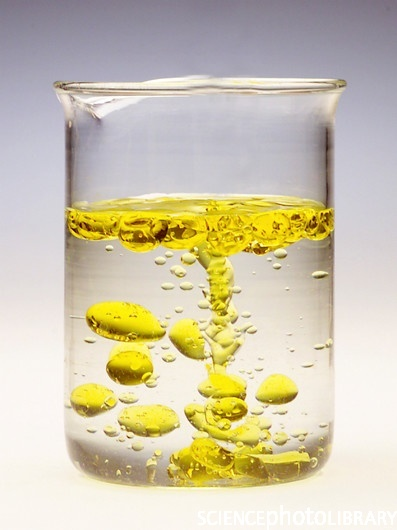
\includegraphics[width=4cm]{oilwater.jpg}
\end{figure}
}
\end{minipage}
&
\begin{minipage}{0.6\textwidth}
\visible<2->{
\begin{figure}[h!]
  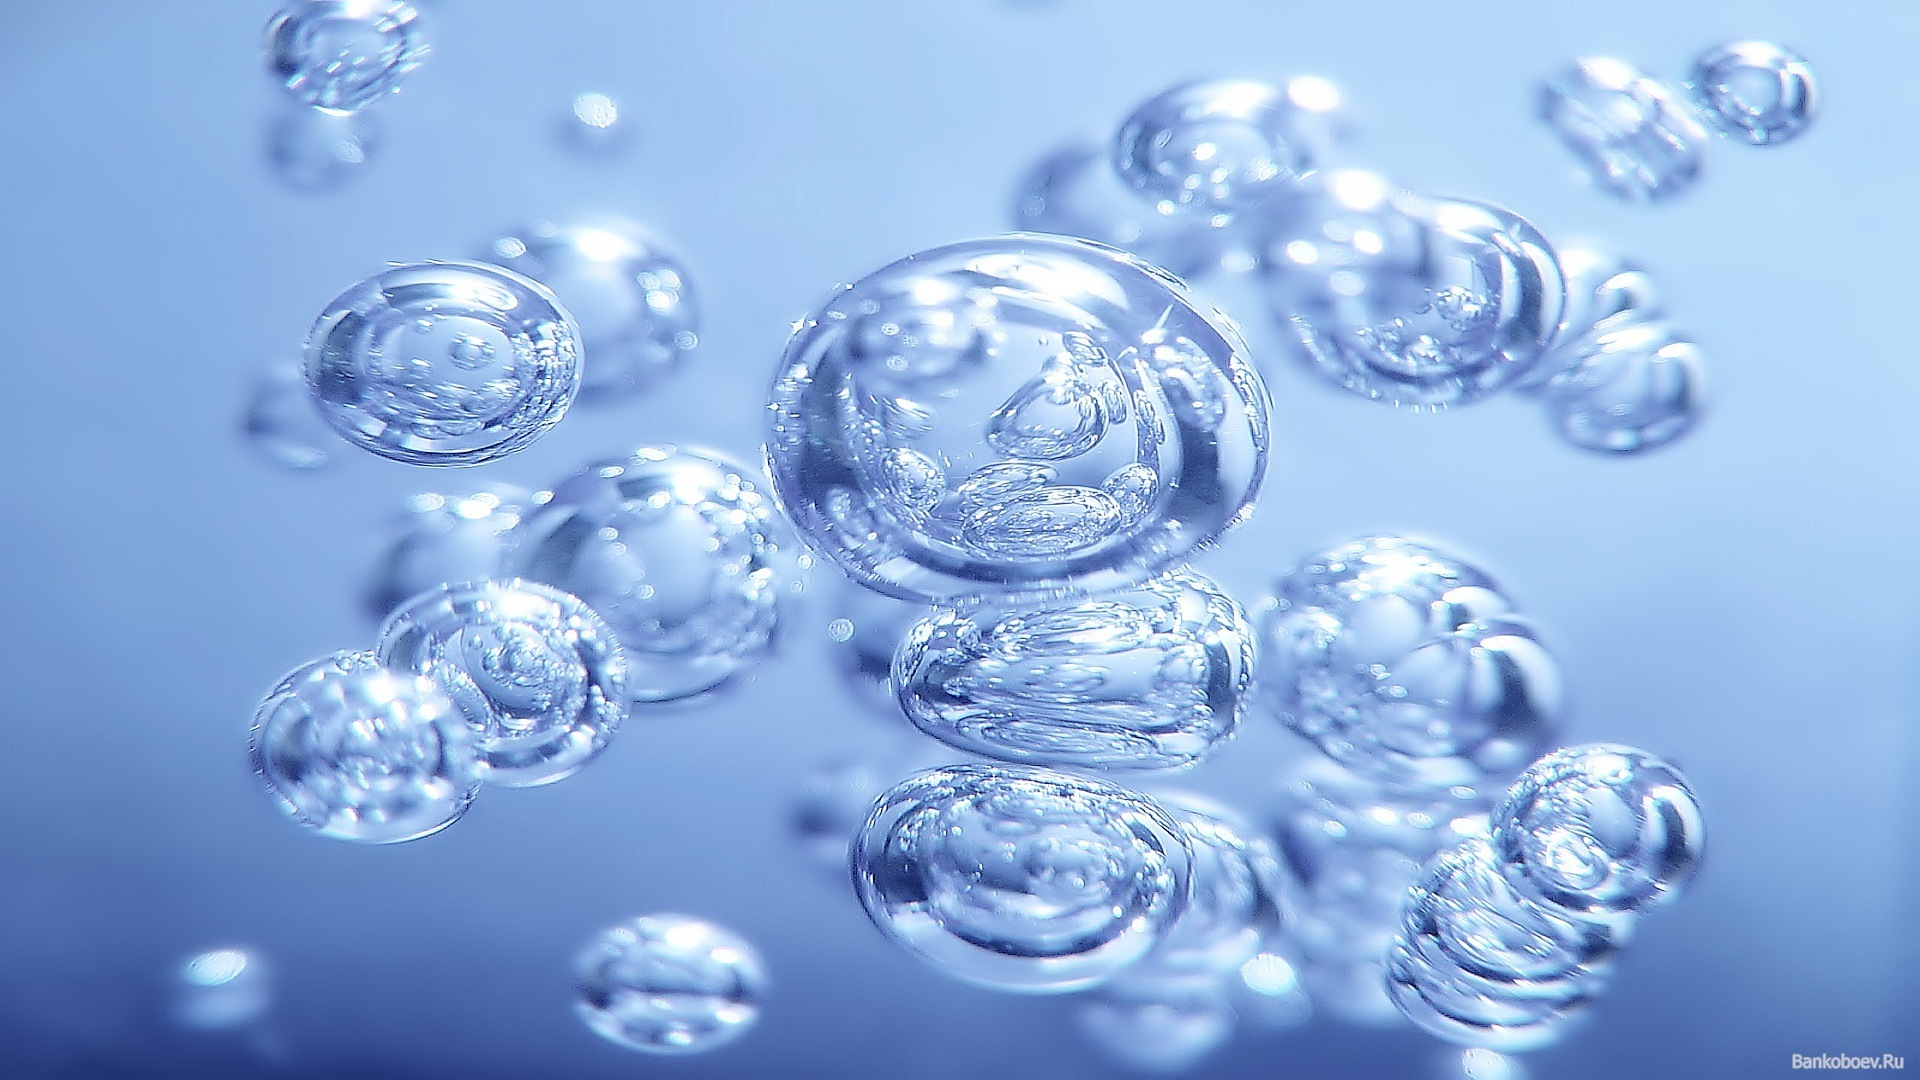
\includegraphics[width=5.5cm]{bubbles.jpg}
\end{figure}
}
\end{minipage}
\end{tabular}


\end{frame}

\section{Mathematic foundation}
\begin{frame}
\frametitle{Macroscopic fluid mechanics}

\begin{itemize}
\item<1-> $N$ immiscible fluids.
\item<2-> Each has own $\rho_i, \nu_i$
\item<3-> Hydrodynamics described by (incompressible) NSE
\end{itemize}
\visible<3->{
$$
\nabla \cdot  \vec v = 0
$$
$$
\frac{\partial \vec v}{\partial t} + \left(\vec  v \cdot \nabla \right) \vec v
=
-\frac{1}{\varrho_i}\nabla p + \nu_i \nabla^2 \vec v $$
}
\end{frame}

\begin{frame}
\frametitle{Mathematic foundation}
\framesubtitle{Interface conditions}
\begin{figure}[h!]
    %\flushright
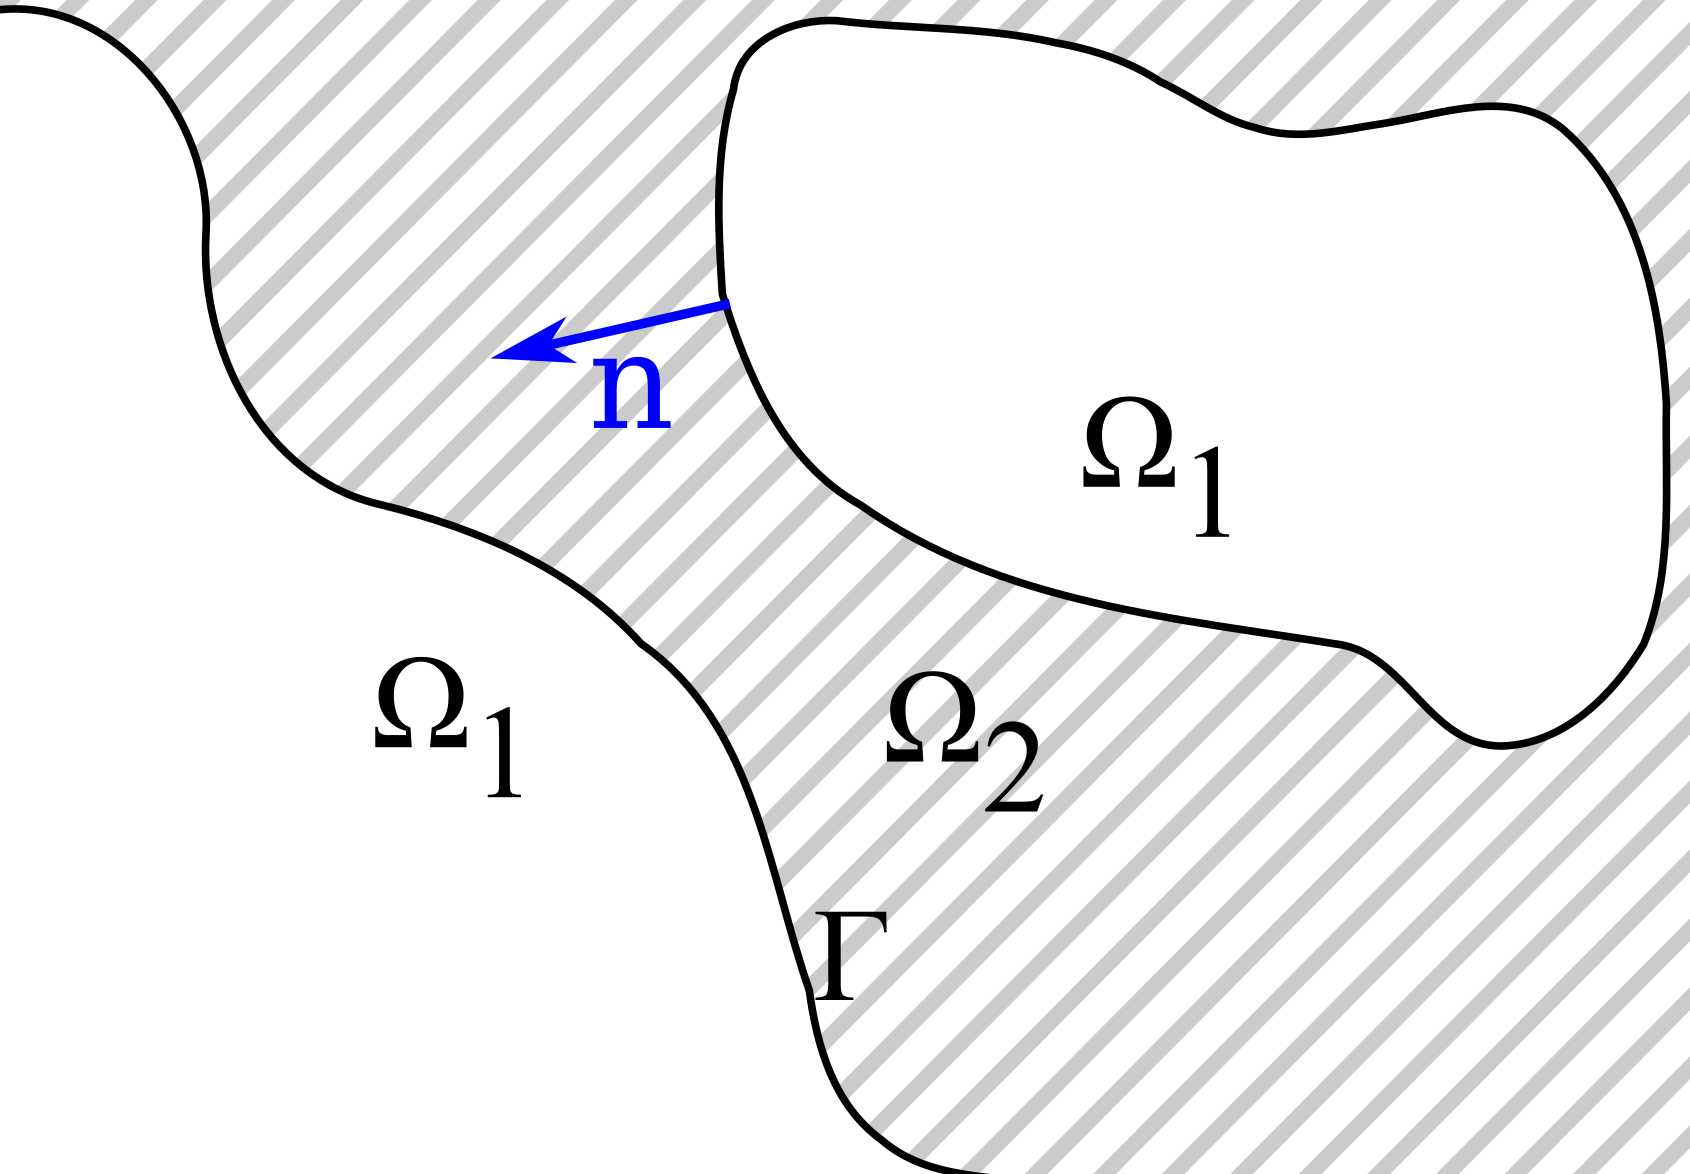
\includegraphics[width=6cm]{skizze.png}
  \caption{Two fluid domains $\Omega_i$ and interface $\Gamma$ inbetween}
\end{figure}
\begin{itemize}
\item<1-> Velocity across interface is $C_0$-continous 
  $$[v] = \lim_{\epsilon \to 0}(\vec v\left(x+\epsilon \vec n\right) -\vec v(x-\epsilon \vec n))=0$$
\end{itemize}
\end{frame}

\begin{frame}
\frametitle{Mathematic foundation}
\framesubtitle{Interface conditions cont'd}
\vspace{-.5cm}
\begin{figure}[h!]
    %\flushright
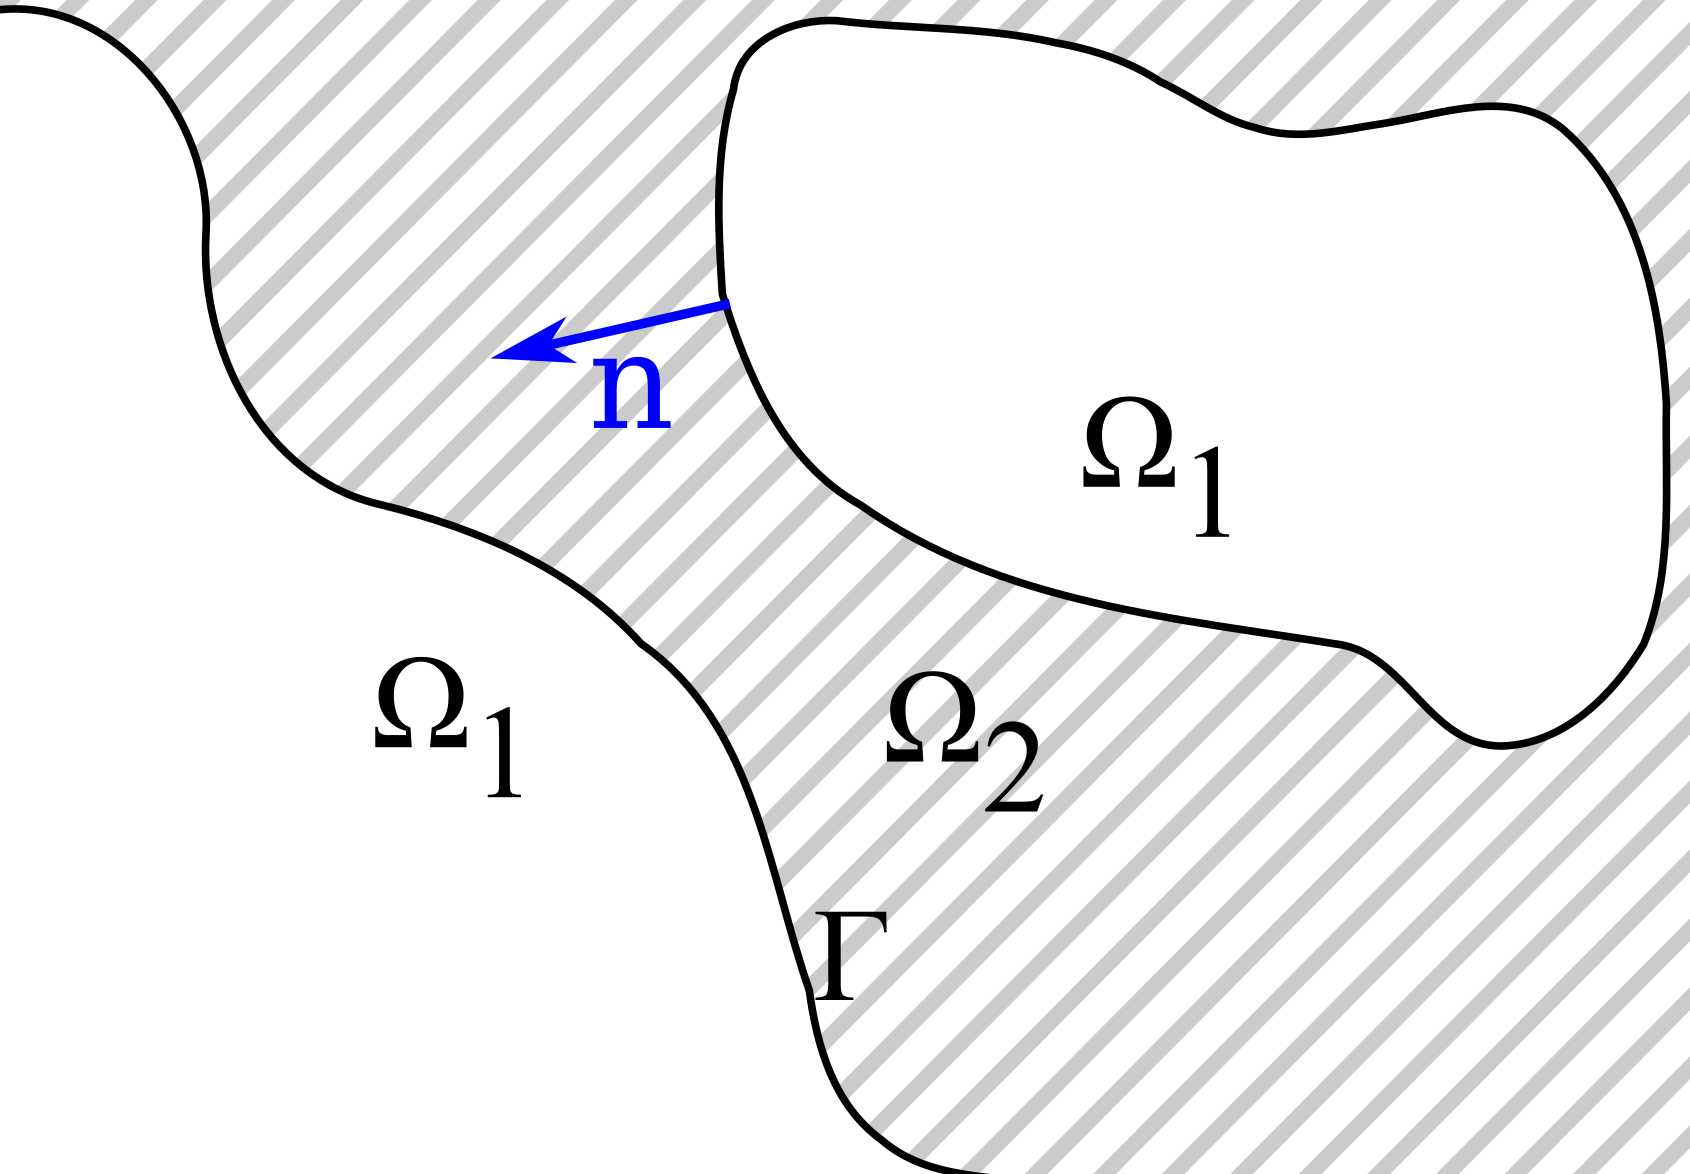
\includegraphics[width=4cm]{skizze.png}
  %\caption{Two fluid domains $\Omega_i$ and interface $\Gamma$ inbetween}
\end{figure}
\vspace{-.5cm}
\begin{itemize}
\item<1->Normal stress is balanced by surface tension $\rightarrow$ pressure jump
  $$[T] \cdot \vec n= \lim_{\epsilon \to 0}(\textbf{T}_2(x+\epsilon \vec n) - \textbf{T}_1(x-\epsilon \vec n)) \cdot \vec n= 2\sigma \kappa \vec n$$
\end{itemize}
\vspace{-.5cm}
\visible<2->{
  where $\textbf{T}_i$ is the stress tensor $\textbf{T}_i=2\nu_i \rho_i \textbf{S}_i -p \mathbb{I}$ and $\kappa$ is the curvature of the interface $\nabla \cdot \vec n$. $\textbf{S}_{ij} = \frac{1}{2}(\partial_{i} v_j+\partial_{j}  v_i)$.
}
\end{frame}

\begin{frame}
To solve the two-phase problem we need to:
\begin{itemize}
\item<1-> solve the flow equations $\rightarrow$ LBM
\item<2-> compute the motion of the interface $\rightarrow$ Level Set Method
\item<3-> couple the two algorithms $\rightarrow$ according BC's % Fuers coupling muessen ja eigentlich nur eine spezielle LBM-Randbehandlung am Interface gemacht werden, und fuer Coupling in die anderere Richtung halt die Geschwindigkeit interpoliert werden
\end{itemize}
\end{frame}

\begin{frame}
\frametitle{Mathematic foundation}
\framesubtitle{Interface capturing}
The interface between fluid phases is captured by a Level-Set Method. 
I.e. a \textit{level set function} $\varphi:= \varphi(x,t) \rightarrow \mathbb{R}$ is tracked through the fluid domain. The interface is given (implicitly) by the zero-isosurface of this function.
It holds:
$$ \frac{\partial \varphi}{\partial t} + \vec v \cdot \nabla \varphi = 0$$
where $\vec v$ is the velocity at the interface, given by NSE.

Benefit of Level-Set Method:
\begin{itemize}
\item<2-> Implicit surface description eases bubble coalescence/breakup in code
\item<3-> High density and viscosity ratios ($>10^3$) possible for simulation
\end{itemize}
\end{frame}

\begin{frame}
\frametitle{Mathematic foundation}
\framesubtitle{Interface implementation (Methods Coupling)}
Hydrodynamics are solved by LBM (D2Q9, SRT for our first test)
\begin{itemize}
\item<1-> Interface becomes a new boundary condition for LBM
$$f_i(x,t+1) = f_{i^*}^{+}(x,t) + 6 \Delta x f_{i}^{*}c_i \cdot \tilde{v} + R_i$$
\item<2-> $\tilde{v}$ is the velocity on the interface along the direction $c_i$
\end{itemize}
\begin{tabular}{l l}
\hspace{-.35cm} \begin{minipage}{0.6\textwidth}
\visible<1->{
\begin{itemize}
\item<3-> $R_i$ ensures the jump conditions of the normal stress and corrects the error terms resulting from the bounce back treatment
\end{itemize}
}
\end{minipage}
&
\begin{minipage}{0.4\textwidth}
\begin{figure}[h!]
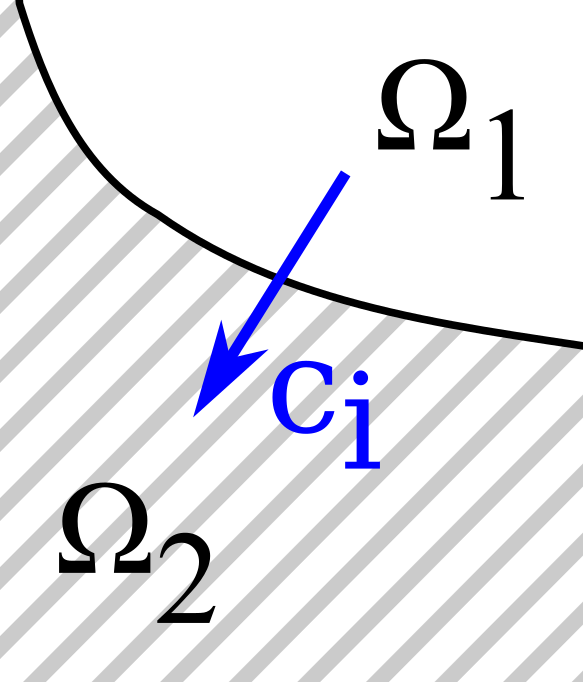
\includegraphics[width=3cm]{skizze2.png}
\end{figure}
\end{minipage}
\end{tabular}
\end{frame}

\begin{frame}
\visible<1->{
$\tilde{v}$ is calculated by linear interpolation:
$$\tilde{v} = q v (x_2,t) + (1-q) v(x_1,t)$$
}
\visible<2->{
$R_i$ consists of several parts:
$$R_i = 6 \Delta x^2 f_{i}^{*} {\Lambda}_i : A$$
}
\visible<3->{
\begin{itemize}
\item<3-> with:
$$ {\Lambda}_i = c_i \otimes c_i - \frac13 {|c_i|}^2 \mathbb{I}$$
$$ A = -q(1-q)[S] - (q - 1/2) S^{2} + O(\Delta x)$$
\item<4-> $S^{(k)}$ velocity gradient at $x_k$
\item<5-> $[S] = \lim_{\epsilon \to 0}(S(x+\epsilon \vec n) -S(x-\epsilon \vec n))$ jump of velocity gradient at the interface. Depends on normal, tangent and curvature.
\end{itemize}
}
\end{frame}

\begin{frame}
\frametitle{Mathematic foundation}
\framesubtitle{Algorithm for LBM with level set}
\begin{itemize}
\item<1-> Create initial interface
\item<2-> Run level set method to calculate surface description
\item<3-> Run LBM for a prescribed number of steps
\item<4-> Run level set method for the same number of steps
\item<5-> Repeat till end of simulation
\end{itemize}
\end{frame}

\section{Results}
\begin{frame}
\frametitle{Validation}
TODO: Hier könnte man Bilder von unserer ersten Simulation zeigen. Leider können wir die Richtigkeit bisher nicht mit Zahlen belegen.
\framesubtitle{Validation setups}
\end{frame}

\section{Outlook}
\begin{frame}
\frametitle{Outlook}
$\rightarrow$ \textit{Conclusion habe ich rausgenommen. Ich wüsste zumindest nicht was wir da reinschreiben könnten. Wenn du was weißt, darfst du das aber sehr gerne wieder einfügen.}

\vspace{.8cm} 
Outlook:
\begin{itemize}
\item<1-> Add correction term to prevent mass loss
\item<2-> Reduce computational effort: Store Level-Set function only in narrow band around interface, Adalsteinsson and Sethian
TODO: Quellen als Footnotes + Uebersichtsfolie
\item<3-> Include thermal flow (simulate e.g. lava lamp) / Include gravity
\end{itemize}

\end{frame}

\begin{frame}
\frametitle{References}
\begin{thebibliography}{etw}
   \bibitem{thoemmes}
     Thömmes, Guido, et al. "A lattice Boltzmann method for immiscible multiphase flow simulations using the level set method." Journal of Computational Physics 228.4 (2009): 1139-1156
   \bibitem{mitchell}
     Mitchell, Ian, A Toolbox of Level Set Methods
\end{thebibliography}
\end{frame}

\end{document}
